\part{L'architecture}
\label{part:archi}

\chapter{La carte du territoire}

\section{Un contrôleur, trois exécutants}

\begin{figure}[htbp]
\centering
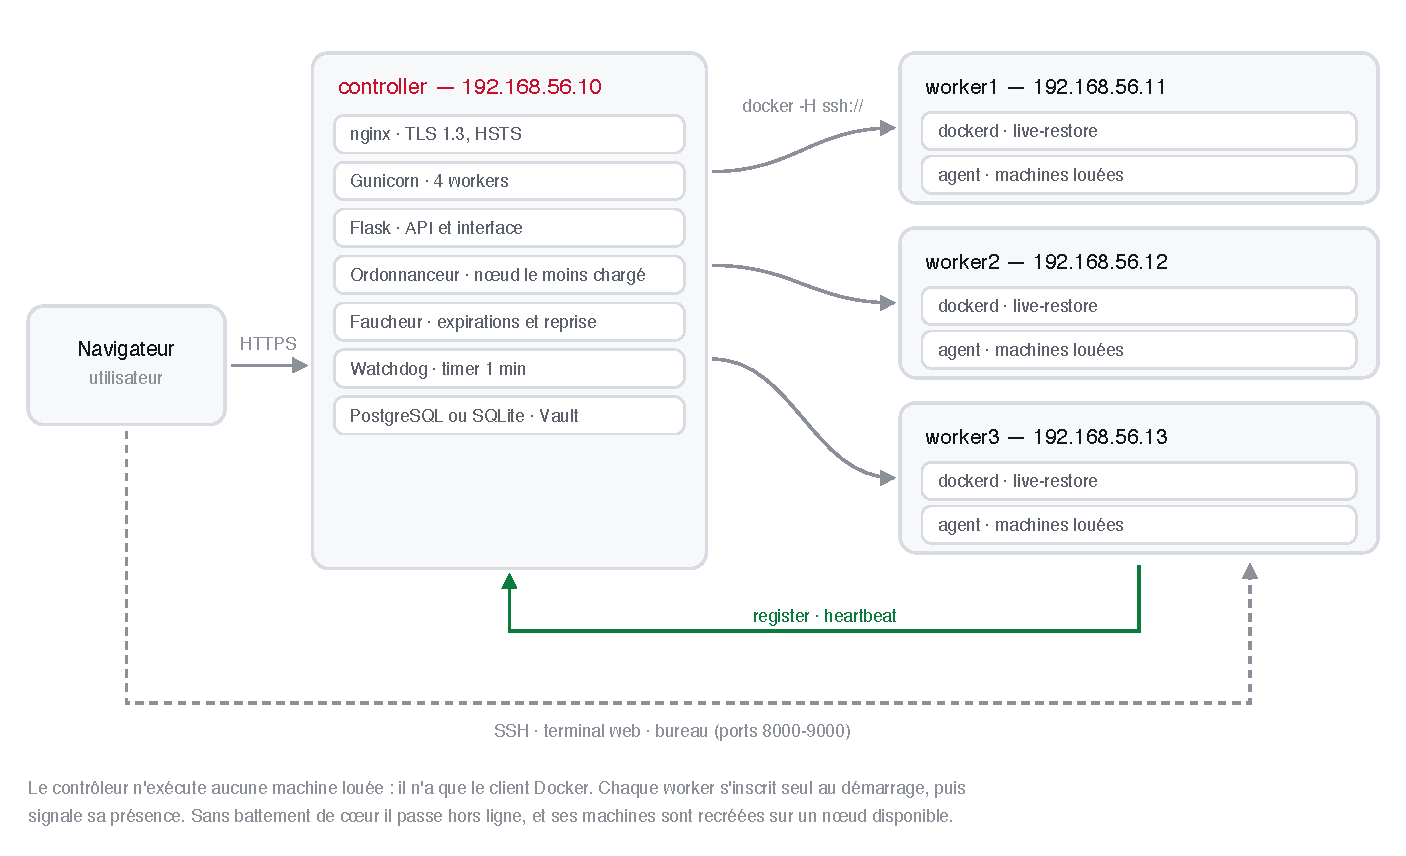
\includegraphics[width=\textwidth]{figures/architecture.pdf}
\caption{L'architecture déployée. Le contrôleur décide, les workers exécutent.}
\label{fig:archi}
\end{figure}

La plateforme se répartit sur quatre machines.

\paragraph{Le contrôleur} (192.168.56.10) porte tout ce qui réfléchit : le site
web, l'API, la base de données, l'ordonnanceur qui choisit où placer une
machine, et le Faucheur qui détruit celles qui ont expiré. Il n'exécute
\emph{aucune} machine louée et n'a même pas de démon Docker --- seulement le
client.

\paragraph{Les workers} (.11, .12, .13) portent tout ce qui exécute : un démon
Docker, les conteneurs loués, et un petit agent qui signale leur présence.

\begin{retenir}
Cette séparation n'est pas décorative. Elle garantit qu'un utilisateur qui
s'échapperait de son conteneur se retrouverait sur un worker --- une machine
sans base de données, sans clés, sans code de la plateforme. Le contrôleur,
lui, n'exécute rien qui vienne de l'extérieur.
\end{retenir}

\section{Comment le contrôleur pilote les workers}

Il existe deux façons de commander un démon Docker distant.

\paragraph{Exposer l'API Docker sur le réseau} (port 2375/2376). C'est simple,
et c'est une très mauvaise idée : qui parle au démon Docker d'une machine en
est root. Une erreur de pare-feu et toute la plateforme est compromise.

\paragraph{Passer par SSH.} Le client Docker sait le faire nativement :

\begin{lstlisting}[language=bash]
docker -H ssh://insacloud@worker1 ps
\end{lstlisting}

Aucun port Docker n'est ouvert. L'authentification est celle de SSH, par clé.
Le compte \cmd{insacloud} du worker n'a pas de mot de passe et n'est
joignable que depuis le contrôleur.

\begin{lstlisting}[language=Python,caption={\fichier{2\_webapp/workers.py} --- le préfixe de commande}]
def docker_command(worker: str = "local") -> list:
    """Prefixe de commande docker pour ce noeud."""
    host = worker_host(worker)
    if host is None:
        return ["docker"]
    return ["docker", "-H", f"ssh://{DOCKER_SSH_USER}@{host}"]
\end{lstlisting}

Toute commande Docker du projet passe par cette fonction. Conséquence
heureuse : le code est le même en mono-hôte (développement) et en cluster
(production). Seul le préfixe change.

\begin{notion}{Le mode mono-hôte}
Si l'inventaire ne déclare aucun worker, \cmd{worker\_host} renvoie
\cmd{None}, le préfixe se réduit à \cmd{docker}, et tout tourne sur la machine
locale. C'est ce qui permet de développer sur un portable sans monter quatre
VM, et c'est ce que fait la pile \cmd{docker compose}.
\end{notion}

\section{Comment le contrôleur apprend l'existence des workers}

C'est le point qui distingue une maquette d'une vraie plateforme :
\textbf{rien n'est écrit en dur}. Le contrôleur ne contient aucune liste
d'adresses de workers.

Chaque worker porte un petit agent qui, au démarrage, se présente au
contrôleur, puis signale régulièrement qu'il est toujours vivant.

\begin{figure}[htbp]
\centering
\begin{tikzpicture}[font=\scriptsize,
  b/.style={draw=grisligne,fill=grisfond,rounded corners=3pt,minimum height=8mm,
            minimum width=2.9cm,align=center},
  f/.style={-{Stealth[length=2mm]},vertok,thick}]
\draw[draw=grisligne,fill=white,rounded corners=4pt] (-1.75,-2.3) rectangle (1.75,2.1);
\node[font=\small\bfseries,insared] at (0,1.75) {contrôleur};
\node[b] at (0,1.0) {base de données};
\node[b] at (0,0.1) {API \texttt{/workers/*}};
\node[b] at (0,-0.8) {ordonnanceur};
\node[b] at (0,-1.7) {Faucheur};

\draw[draw=grisligne,fill=grisfond,rounded corners=4pt] (5.2,-0.85) rectangle (8.4,0.95);
\node[font=\small\bfseries] at (6.8,0.6) {worker2};
\node at (6.8,0.1) {agent};
\node[gristexte] at (6.8,-0.45) {dockerd};

\draw[f] (5.15,0.55) -- (1.85,0.55)
  node[midway,above,vertok]{1. \texttt{POST /workers/register}}
  node[midway,below,gristexte]{nom, IP, cœurs, mémoire};
\draw[f] (5.15,-0.2) -- (1.85,-0.2)
  node[midway,above,vertok]{2. \texttt{POST /workers/heartbeat}}
  node[midway,below,gristexte]{toutes les 30 s};
\draw[-{Stealth[length=2mm]},orangepartiel,thick,dashed] (1.85,-1.7) -- (5.15,-1.7)
  node[midway,above,orangepartiel,align=center]{3. plus de battement pendant 90 s};
\node[orangepartiel] at (6.8,-1.7) {OFFLINE};
\end{tikzpicture}
\caption{L'inscription spontanée. Allumer un worker suffit à l'ajouter au
parc ; l'éteindre suffit à l'en sortir.}
\end{figure}

\begin{retenir}
Ajouter un quatrième worker ne demande de modifier aucun fichier sur le
contrôleur. On l'allume, il s'inscrit, l'ordonnanceur commence à lui envoyer
des machines. C'est la \textbf{Fonctionnalité 7} du cahier des charges, et
c'est ce qui rend le parc élastique.
\end{retenir}

\chapter{Le modèle de données}
\label{chap:modele}

\begin{figure}[htbp]
\centering
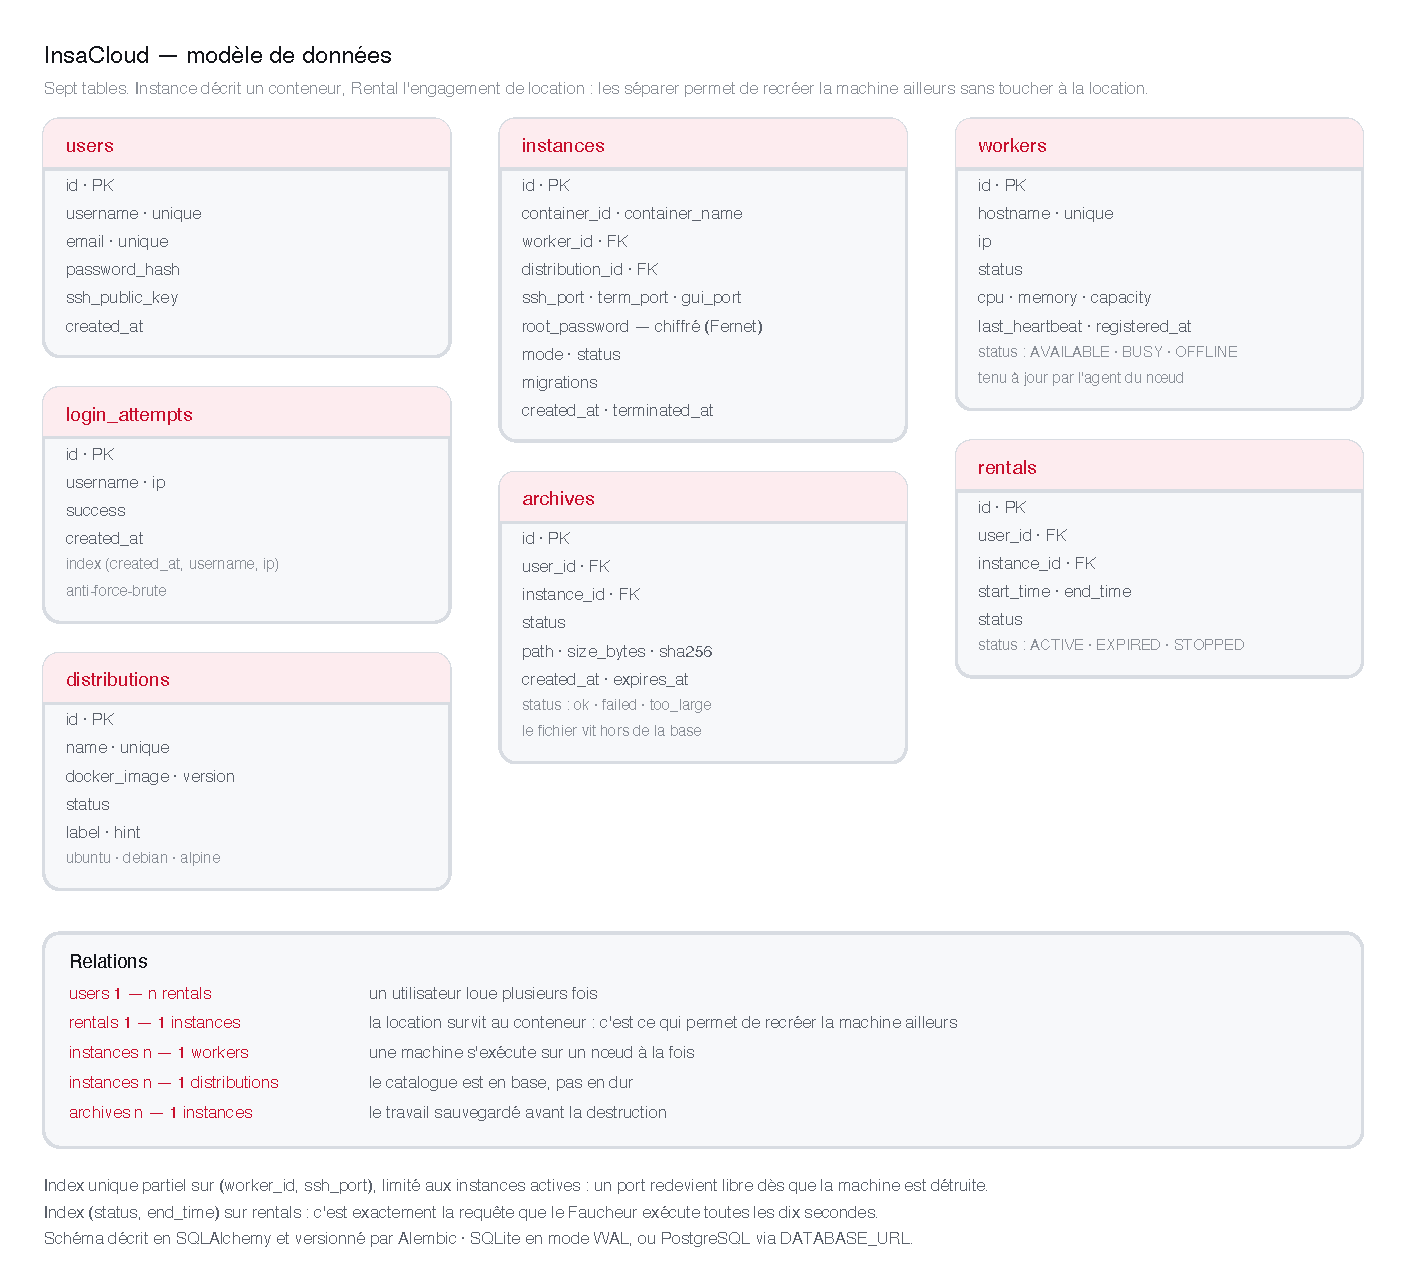
\includegraphics[width=\textwidth]{figures/base-de-donnees.pdf}
\caption{Les sept tables. La séparation \texttt{instances} / \texttt{rentals}
est la décision qui structure tout le reste.}
\label{fig:bdd}
\end{figure}

\section{Pourquoi séparer la machine de la location}

C'est le choix le moins évident et le plus important du projet.

On pourrait n'avoir qu'une table : une ligne par location, contenant à la fois
l'engagement (quel utilisateur, jusqu'à quand) et la machine (quel conteneur,
quel port, sur quel nœud). C'est plus court, et c'est ce qu'on écrit
naturellement.

Cela rend la reprise après panne \textbf{impossible}.

Quand un nœud tombe, il faut recréer la machine ailleurs : nouveau conteneur,
nouveau port, nouveau nœud, nouveau mot de passe. Mais la location, elle, ne
doit pas bouger : l'utilisateur a réservé trente minutes, il doit garder ses
trente minutes. Avec une table unique, on ne peut pas changer l'un sans
toucher à l'autre.

\begin{description}
\item[\texttt{Instance}] décrit un conteneur : son identifiant Docker, son
  nœud, ses ports, son mot de passe chiffré, son état.
\item[\texttt{Rental}] décrit l'engagement : quel utilisateur, de quand à
  quand, actif ou non.
\end{description}

La reprise change l'\texttt{Instance} et ne touche pas au \texttt{Rental}.

\begin{retenir}
Quand une table mélange « ce qui est promis » et « ce qui l'exécute », toute
panne devient visible par l'utilisateur. Séparer les deux est ce qui permet de
réparer sans rien lui reprendre.
\end{retenir}

\section{Les sept tables}

\begin{center}
\small
\begin{tabularx}{\textwidth}{@{}lX@{}}
\toprule
\textbf{Table} & \textbf{Ce qu'elle porte} \\
\midrule
\texttt{users} & comptes : identifiant, empreinte du mot de passe, clé SSH publique \\
\texttt{login\_attempts} & tentatives de connexion, pour le verrouillage anti-force-brute \\
\texttt{distributions} & le catalogue : Ubuntu, Debian, Alpine --- en base, pas en dur \\
\texttt{workers} & le parc : nom, adresse, état, charge, dernier battement de cœur \\
\texttt{instances} & les conteneurs : identifiant Docker, nœud, ports, secret chiffré \\
\texttt{rentals} & les locations : utilisateur, début, fin, état \\
\texttt{archives} & le travail sauvegardé avant destruction \\
\bottomrule
\end{tabularx}
\end{center}

\section{Deux index qui portent une règle métier}

Un index n'est pas qu'une optimisation : il peut imposer une contrainte que le
code aurait du mal à garantir seul.

\begin{lstlisting}[language=Python,caption={\fichier{2\_webapp/models.py} --- l'unicité du port}]
__table_args__ = (
    Index("idx_instances_status", "status"),
    # Index unique PARTIEL : deux machines actives ne peuvent pas partager un
    # port sur le meme noeud. La clause « where » le limite aux instances en
    # cours, donc un port redevient libre des que la machine est detruite.
    Index("uq_worker_port_actif", "worker_id", "ssh_port", unique=True,
          sqlite_where=text("status = 'running'"),
          postgresql_where=text("status = 'running'")),
)
\end{lstlisting}

\begin{notion}{Index unique partiel}
Un index unique classique interdirait deux fois le même port \emph{pour
toujours} : les machines détruites continueraient de réserver le leur. La
clause \cmd{WHERE} restreint la contrainte aux lignes qui comptent.

Sans cela, deux requêtes simultanées pourraient choisir le même port libre et
créer deux conteneurs en conflit --- une \emph{situation de compétition} que
le code applicatif ne peut pas écarter seul, car entre « ce port est libre »
et « je le prends » il s'écoule toujours un instant.
\end{notion}

Le second index sert le Faucheur :

\begin{lstlisting}[language=Python]
__table_args__ = (Index("idx_rentals_end", "status", "end_time"),)
\end{lstlisting}

C'est exactement la requête qu'il exécute toutes les dix secondes : « les
locations actives dont la date de fin est passée ». Sans index, chaque passage
relirait toute la table.

\chapter{Le cycle de vie d'une machine}
\label{chap:cycle}

\begin{figure}[htbp]
\centering
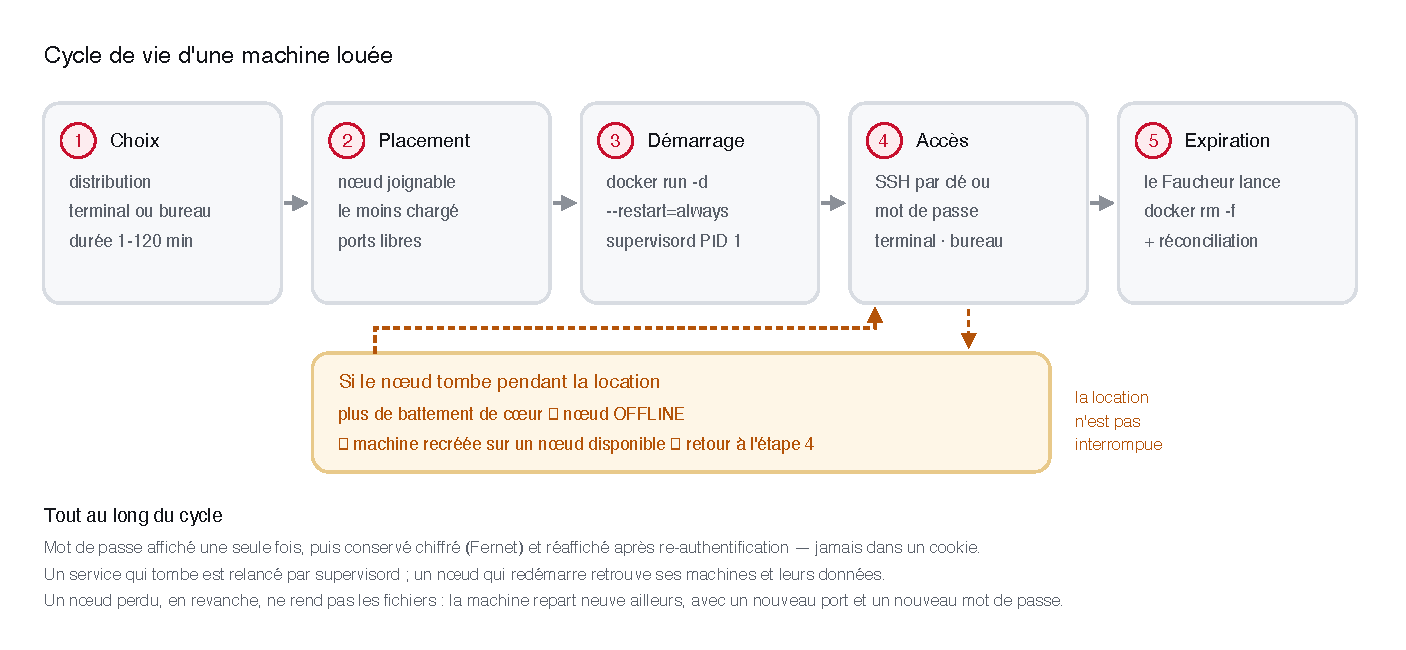
\includegraphics[width=\textwidth]{figures/cycle-de-vie.pdf}
\caption{De la demande à l'expiration, avec la branche de reprise si un nœud
tombe pendant la location.}
\label{fig:cycle}
\end{figure}

\section{Les cinq étapes}

\begin{enumerate}
\item \textbf{Choix.} L'utilisateur sélectionne une distribution, un mode
  (terminal ou bureau) et une durée de 1 à 120 minutes. Les trois valeurs sont
  validées côté serveur --- ce qui vient du navigateur n'est jamais cru.
\end{enumerate}

\begin{figure}[htbp]
\centering
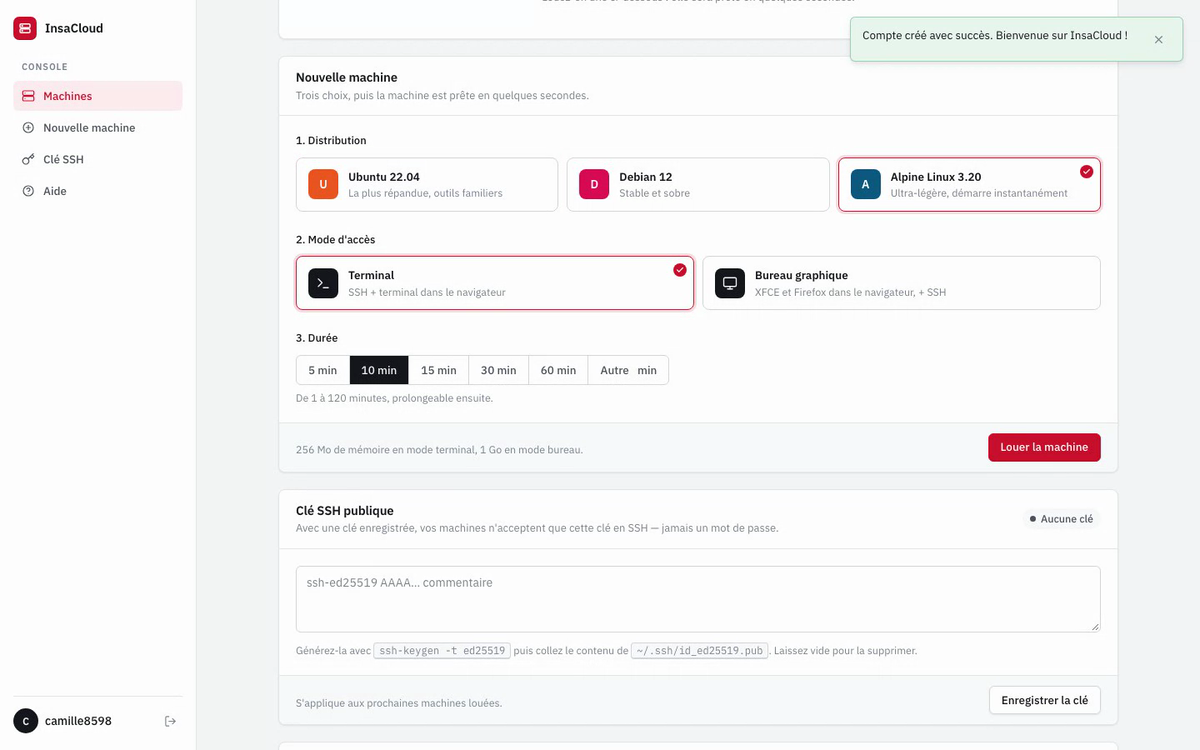
\includegraphics[width=0.84\textwidth]{../docs/04-choix-machine.png}
\caption{L'étape 1 vue par l'utilisateur. Une distribution dont l'image n'est
pas construite sur le parc n'apparaît pas : le catalogue interroge Docker
avant d'afficher un choix.}
\end{figure}

\begin{enumerate}
\setcounter{enumi}{1}
\item \textbf{Placement.} L'ordonnanceur retient le nœud joignable le moins
  chargé, puis réserve un port libre dans la plage 8000--9000.
\item \textbf{Démarrage.} \cmd{docker run -d --restart=always -p <port>:22}
  crée le conteneur ; \cmd{supervisord} y démarre en PID 1 et lance les
  services du mode choisi.
\item \textbf{Accès.} L'utilisateur reçoit une commande SSH et, selon le mode,
  l'adresse d'un terminal web ou d'un bureau. Le mot de passe root est affiché
  \emph{une seule fois}.
\item \textbf{Expiration.} Le Faucheur détruit la machine à l'échéance et
  libère le port.
\end{enumerate}

\section{La branche qui fait la différence}

Si le nœud tombe \emph{pendant} la location, l'agent cesse de battre. Au bout
de 90 secondes sans nouvelle, le contrôleur déclare le nœud hors ligne et
recrée ses machines sur un nœud disponible. L'utilisateur garde sa location,
sa durée et son droit d'accès ; il reçoit un nouveau port et un nouveau mot de
passe.

\begin{piege}{La reprise ne rend pas les fichiers}
Il faut le dire clairement, parce que c'est une limite assumée et pas un
oubli : les fichiers créés dans l'ancienne machine vivaient dans sa couche
inscriptible, sur un nœud devenu injoignable. Sans stockage partagé entre les
nœuds, ils sont perdus. Seul le \emph{service} repart.

Un volume répliqué (NFS, Ceph) changerait la nature du projet et son
périmètre. C'est un choix documenté, pas une négligence.
\end{piege}

\section{Trois niveaux de résilience}

La haute disponibilité se joue à trois échelles emboîtées, et c'est ce
qu'attend la \textbf{Fonctionnalité 13}.

\begin{center}
\small
\begin{tabularx}{\textwidth}{@{}llX@{}}
\toprule
\textbf{Échelle} & \textbf{Mécanisme} & \textbf{Ce qu'il rattrape} \\
\midrule
Dans la machine & \cmd{supervisord} & un service meurt (sshd, ttyd, VNC) : il est relancé \\
Sur le nœud & \cmd{--restart=always} & supervisord meurt : Docker relance le conteneur \\
Sur le nœud & \cmd{live-restore} & le démon Docker redémarre : les conteneurs continuent \\
Dans le parc & battement de cœur & le nœud entier tombe : les machines repartent ailleurs \\
\bottomrule
\end{tabularx}
\end{center}

\begin{figure}[htbp]
\centering
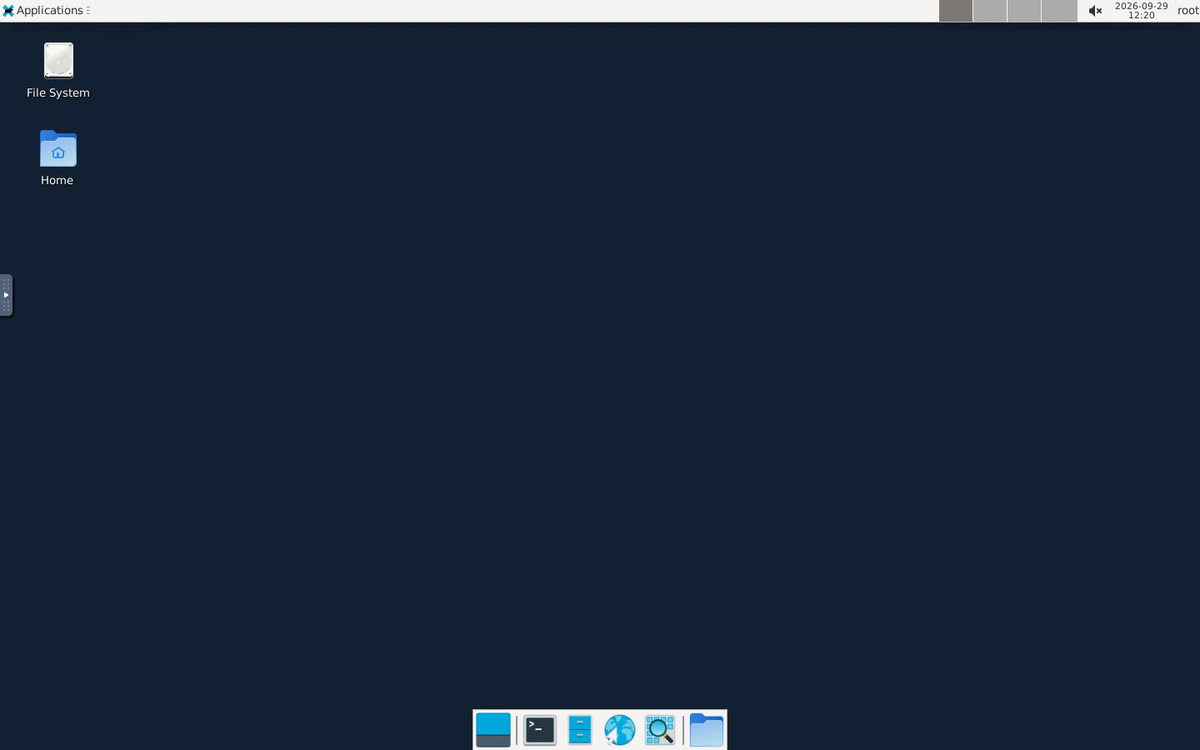
\includegraphics[width=0.84\textwidth]{../docs/10-machines-en-cours.png}
\caption{Deux machines en cours, une par mode d'accès. Le temps restant est
calculé à l'affichage ; c'est le Faucheur, et non la page, qui décide de la
destruction.}
\end{figure}

\begin{notion}{\texttt{live-restore}}
Par défaut, redémarrer le démon Docker arrête tous ses conteneurs. L'option
\cmd{live-restore} les laisse tourner pendant ce redémarrage. Pour une
plateforme de location, c'est la différence entre « une mise à jour de Docker
coupe tous les clients » et « personne ne s'en aperçoit ».
\end{notion}
